\documentclass[10pt, a4paper]{article}
\usepackage{float} % display graphics at the demanded place
\usepackage{hyperref} % display table des matières
\usepackage{subcaption} % authorize subfigure
\usepackage{booktabs}
\usepackage[utf8]{inputenc}
\usepackage[T1]{fontenc}
%\usepackage[french]{babel} %casse tout chez moi
\usepackage{graphicx}
\usepackage{rotating}

%élargi un peu pour que les diagrammes soient pas minuscules ou mal alignés
\evensidemargin=0in
\oddsidemargin=0in
\textwidth=6.5in

\graphicspath{{Diagrammes/}}


\title{\LARGE{INFO-F-109 : Projet d'informatique 2 }\\
       \textbf{Software requirement document\\
	   Pawn Hub}}
\author{Huwart Maxence, Boonen Jacques\\
		Pham Hong Phuc, Duc Nguyen, Caroline Forest\\
		Antunes Andre, Romain Mardulyn}
\date{17 Décembre 2018}
\begin{document}
	\maketitle
	\newpage
	\renewcommand{\contentsname}{Table des Matières}
	\tableofcontents %do a table of content automatically
	\newpage
	\section{Introduction}
		\subsection{Description du Projet}
			\paragraph{}Ce projet aura pour but de recréer un grand classique des jeux de plateau: les échecs. Le jeu sera jouable via un mode multijoueurs. Le joueur pourra jouer au mode classique ou à une de ses variantes telles que  {\itshape AliceChess, DarkChess} et {\itshape HordeChess} que nous décrirons plus tard. De plus, il aura également la possibilité de créer un compte à partir duquel il pourra effectuer plusieurs actions qui seront détaillées ci-dessous. Néanmoins, le joueur pourra lancer une partie en tant que {\itshape visiteur} mais ne bénéficiera pas des avantages liés à la possession d'un compte.
			\subsection{Fonctionnement du Jeu d'Échec}
			\subsubsection{Règles du Jeu\footnote{Wikipedia}} Chaque joueur possède au départ un roi, une dame, deux tours, deux fous, deux cavaliers et huit pions. Le but du jeu est d'infliger à son adversaire un échec et mat, une situation dans laquelle le roi d'un joueur est en prise sans qu'il soit possible d'y remédier.
			\subsubsection{Les Pièces}
			\begin{description}
		  \item[Le Pion :] Depuis sa position initiale, le pion peut avancer d'une ou 2 cases en avant, ensuite d'une case en avant uniquement. Néanmoins, le pion prend une autre pièce en diagonale. Également, lorsque le pion arrive à la dernière rangée, il effectue une promotion et est remplacé par n'importe quelle autre pièce, à part le roi, au choix du joueur. De plus, il peut également effectuer la prise en passant qui est expliquée dans le glossaire.
			\item[La Tour :] La tour peut se déplacer d'un nombre quelconque de cases sur les rangées et les colonnes.
			\item[Le Fou :] Le fou peut se déplacer uniquement en diagonale d'un nombre quelconque de cases.
			\item[La Reine :] La reine peut se déplacer dans toutes les directions d'un nombre quelconque de cases.
			\item[Le Roi :] Le roi peut se déplacer dans toutes les directions d'une case uniquement. Il peut également effectuer un roque qui est expliqué dans le glossaire.
			\item[Le Cavalier :] Le cavalier se déplace en "L", voir image ci-dessous.
			\begin{figure}[b]
			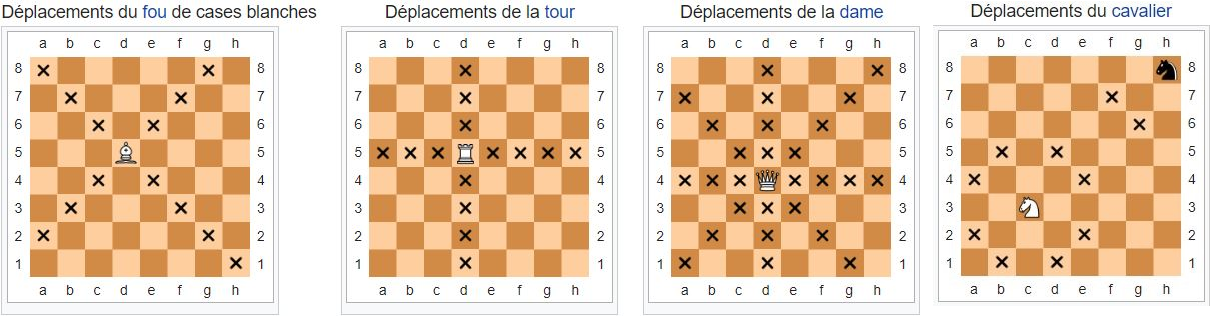
\includegraphics[scale=0.50]{pieces_move.png}
			\caption{Image provenant de Wikipedia}
			\end{figure}
			\end{description}
			\clearpage
			
			\subsection{Les Modes de Jeu}
				\subsubsection{Classique}
					\paragraph{}Le jeu d'échecs classique, où le but est de mettre le roi adverse en échec sans qu'il ait la possibilité au tour suivant de ne plus l'être.
				\subsubsection{Alice Chess}
					\paragraph{}Variante du jeu d'échecs jouée en utilisant 2 boards. Après chaque coup, la pièce déplacée est téléportée sur la case où elle a été placée mais de l'autre board. Un coup n'est valide que si la case où doit se téléporter la pièce ne comporte aucune pièce. À part cela, le jeu se déroule selon les règles habituelles du jeu d'échecs.
				\subsubsection{Dark Chess}
					\paragraph{}Variante du jeu d'échecs où le joueur ne voit que ses propres pièces et les cases où il peut légalement les déplacer. Le but des joueurs est de prendre le roi adverse. Contrairement aux règles classiques, le roi d'un joueur peut être en échec à la fin de son tour. De plus il n'y a pas de prises en passant possible. À part cela, le jeu se déroule selon les règles habituelles du jeu d'échecs.
				\subsubsection{Horde Chess}
					\paragraph{} Variante du jeu d'échecs où le joueur noir possède 32 pions et l'autre la collection standard du jeu d'échecs traditionnel. Le but du joueur noir est le but du jeu classique mais le but du joueur blanc est de prendre tous les pions du joueur noir. À part cela, le jeu se déroule selon les règles habituelles du jeu d'échecs.

			\subsection{Fonctionnalités pour Utilisateur Enregistré et Utilisateur Non-Enregistré}Depuis le menu principal, les joueurs pourront accéder à l'option {\itshape View Rules} à travers lequel ils pourront lire en détail les règles du jeu d'échecs et de ses variantes. Les joueurs lanceront une partie via l'option {\itshape Game}. Lors d'une partie, ils pourront s'envoyer des messages via un chat dédié.

			\subsection{Fonctionnalités pour Utilisateur Enregistré}Les joueurs pourront communiquer via un chat global. Dans le système de matchmaking, ils auront le choix entre affronter un ami ou un joueur aléatoire parmi ceux qui sont connectés et libres\footnote{ne se trouvant pas en partie.}. À travers le menu principal, les utilisateurs accéderont à plusieurs sous-menus tels que {\itshape View Ranking, View Rules, View Statistics, Friends List}.%rajouter d'autres fonctionnalités au besoin.

		\subsection{Glossaire} Par souci de clarté et de lisibilité, toutes les informations relatives aux règles et au fonctionnement officiels des échecs et de ses variantes ne seront pas parcourues ci-dessous.
		\begin{description}
		\item[Un utilisateur non-enregistré :] Joueur ne s'étant pas identifié au système via un compte.
		\item[Un utilisateur enregistré :] Joueur s'étant identifié au système via un compte.
		\item[Joueur :] Utilisateur en partie.
		\item[Matchmaking :] Système qui met en relation 2 joueurs avant le lancement d'une partie.
		\item[Chat :] Système de communication par messages instantanés entre deux joueurs.
		\item[AliceChess :] Variante du jeu d'échec jouée en utilisant 2 plateaux. Lorsqu'un coup est joué, la pièce est déplacée à la case correspondante mais dans l'autre plateau. À part cela, le jeu se déroule selon les règles habituelles du jeu d'échecs .
		\item[DarkChess :] Variante du jeu d'échec où le joueur ne voit que ses propres pièces et les cases où il peut légalement les déplacer.
		\item[HordeChess :] Variante du jeu d'échec où un joueur possède 32 pions et l'autre la collection standard du jeu d'échec traditionnel.
		\item[Le Roque :] Le roque consiste à déplacer en un seul coup le roi et l'une des tours. On déplace d'abord le roi de deux cases vers la tour puis, avec la même main, on fait passer la tour de l'autre côté, juste à côté du roi (voir le diagramme ci-dessous). Les conditions suivantes sont nécessaires pour pouvoir roquer : aucune pièce ne se trouve entre le roi et la tour concernée, le roi et la tour concernée n'ont encore jamais joué et le roi n'est pas en échec ;
la case traversée par le roi n'est contrôlée par aucune pièce adverse\footnote{source Wikipedia}.
		\item[La Prise en Passant:] Au jeu d’échecs, la prise en passant est une possibilité particulière de capturer un pion. Lorsqu’un pion se trouve sur la cinquième rangée1 et que l’adversaire avance de deux cases un pion d’une colonne voisine (les deux pions se retrouvent alors côte-à-côte sur la même rangée), le premier pion peut prendre le second. Pour effectuer la prise en passant, le joueur avance son pion en diagonale sur la sixième rangée et la colonne du pion adverse, et ôte ce dernier de l’échiquier\footnote{source Wikipedia}
		\begin{figure}[b]
		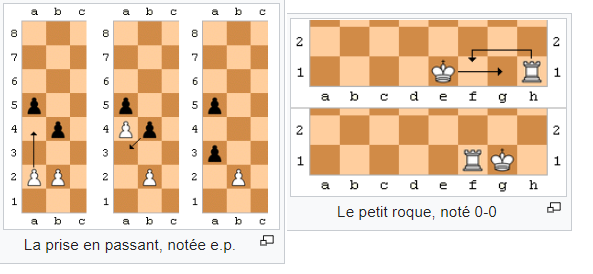
\includegraphics[scale=1]{roque_prise_passant.png}
		\caption{Image provenant de Wikipedia}
		\end{figure}
		
		\end{description}
		\clearpage

		\subsection{Historique des Modifications}

		\begin{table}[h!]

			\centering

			\begin{tabular}{|c|c|c|p{50mm}|}
				\hline
				 \textbf{version} & \textbf{date} & \textbf{auteur}  & \textbf{description} \\ \hline
				 1 & 4/12 & Pham Hong Phuc & Création du SRD + ajout structure\\ \hline
				 1.1 & 6/12 & Caroline Forest & Ajout de diagrammes UML\\ \hline
				 1.2 & 8/12 & Boonen Jacques & 1.Introduction\\ \hline
				 1.3 & 11/12 & Huwart Maxence & Besoins systèmes\\ \hline
				 1.4 & 12/12 & Mardulyn Romain & Explication des différent modes de jeu\\ \hline
				 1.5 & 12/12 & Antunes André & Explication des options durant une partie\\ \hline
         1.6 & 12/12 & Nguyen Duc & Modification des diagrammes de séquence\\ \hline
         1.7 & 13/12 & Pham Hong Phuc & Correction et réajustement \\ \hline
				 1.8 & 12/02 & Boonen Jacques & Fonctionnement du jeu + ajout images \\ 
				 1.9 & 13/02 & Boonen Jacques & Déroulement d'une partie \\ 
				\hline
\end{tabular}
			\caption*{Historique des modifications}
			\end{table}
%fin du tableau
\clearpage

%BESOINS UTILISATEURS%

\section{Besoins Utilisateurs : Fonctionnels}


\subsection{Connexion}

\begin{figure}[ht]
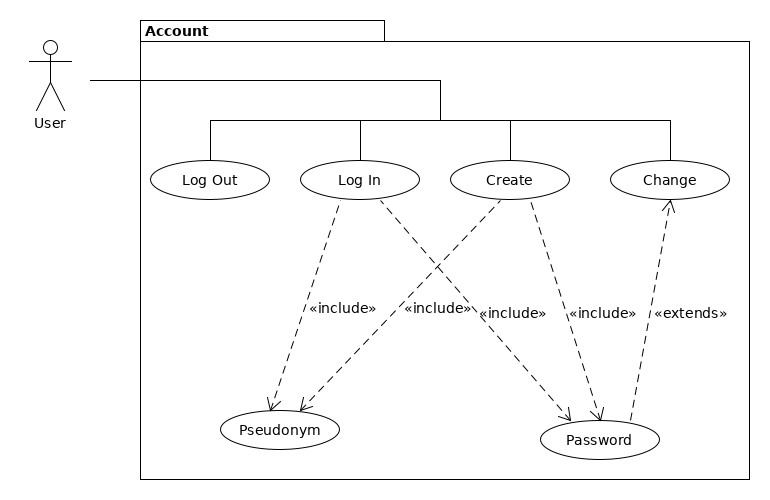
\includegraphics[scale=0.5]{UC_connexion.png}
\caption{Diagramme de \textit{use case} des actions possibles d'un utilisateur quant à son identification}
\label{UC_co} %UseCase_connexion
\end{figure}

\subsubsection{S'identifier}
\textbf{Acteur :} \textit{User}.\\
\textbf{Relations avec d'autres cas d'utilisation :} Néant.\\
\textbf{Pré-conditions :} Le \textit{user} doit avoir sélectionné le sous-menu \textit{Connexion} puis l'option {\itshape Log In} dans le menu principal du jeu.\\
\textbf{Post-conditions :} Le \textit{user} doit encoder un nom d'utilisateur et un mot de passe d'un compte déjà existant dans le système. \\
\textbf{Cas général :} Après s'être identifié, le \textit{user} peut profiter de tous les sous-menus du menu principal.\\
\textbf{Cas exceptionnels :} Si un utilisateur est déjà connecté sur un compte, un autre joueur ne peut se connecter sur ce compte. Également, si l'utilisateur encode mal ses identifiants, le système lui renvoie un message d'erreur afin qu'il les réécrive correctement.



\subsubsection{Créer un Compte}
\textbf{Acteur :} \textit{User}.\\
\textbf{Relations avec d'autres cas d'utilisation :} Néant.\\
\textbf{Pré-conditions :} Le \textit{user} doit avoir sélectionné le sous-menu \textit{Connexion} puis l'option {\itshape Create} dans le menu principal du jeu.\\
\textbf{Post-conditions :} Le \textit{user} doit encoder un nom d'utilisateur et un mot de passe afin de créer son compte.\\
\textbf{Cas général :} Un nom d'utilisateur et un mot de passe correspondant sont encodés dans la base de données du système.\\
\textbf{Cas exceptionnels :} Si le nom d'utilisateur encodé est déjà dans la base de données, l'utilisateur doit en réencoder un nouveau.



\subsection{Menu Principal}

\begin{figure}[ht]
\begin{center}
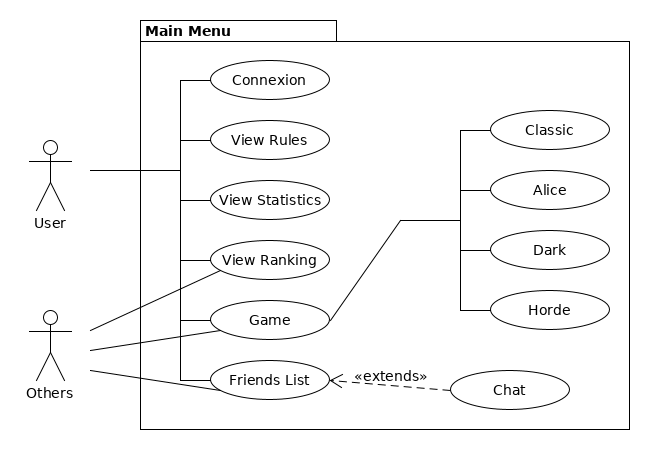
\includegraphics[scale=0.5]{UC_mainmenu.png}
\caption{Diagramme de \textit{use case} des actions possibles d'un utilisateur}
\label{UC_menu} %UseCase_menu
\end{center}
\end{figure}

\subsubsection{Jouer}
\textbf{Acteur :} \textit{User}.\\
\textbf{Relations avec d'autres cas d'utilisation :} Modes de jeu proposés (\textit{Classic}, \textit{Alice}, \textit{Dark} ou \textit{Horde}).\\
\textbf{Pré-conditions :} Le \textit{user} doit avoir sélectionné l'option \textit{Game} dans le menu principal du jeu.\\
\textbf{Post-conditions :} Le  \textit{user} sélectionne un mode de jeu parmi ceux proposés (\textit{Classic},\textit{Alice}, \textit{Dark} ou \textit{Horde}).\\
\textbf{Cas général :} Le  \textit{user} peut sélectionner un mode de jeu parmi ceux proposés (\textit{Classic},\textit{Alice}, \textit{Dark} ou \textit{Horde}), ce qui lance une requête de \textit{matchmaking} (voir Figure \ref{SD_matchmaker}) au serveur.\\
\textbf{Cas exceptionnels :} Néant.



\subsubsection{Voir les Règles}
\textbf{Acteur :} \textit{User}.\\
\textbf{Relations avec d'autres cas d'utilisation :} Néant.\\
\textbf{Pré-conditions :} Le \textit{user} doit avoir sélectionné l'option \textit{View Rules} dans le menu principal du jeu.\\
\textbf{Post-conditions :} Le \textit{user} accède aux règles du jeu.\\
\textbf{Cas général :} Le \textit{user} peut consulter les règles du jeu en envoyant une requête au serveur.\\
\textbf{Cas exceptionnels :} Néant.

\subsubsection{Voir les Statistiques Personnelles}
\textbf{Acteur :} \textit{User}.\\
\textbf{Relations avec d'autres cas d'utilisation :} Néant.\\
\textbf{Pré-conditions :} Le \textit{user} doit avoir sélectionné l'option \textit{View Statistics} dans le menu principal du jeu.\\
\textbf{Post-conditions :} Le \textit{user} accède à ses statistiques personnelles.\\
\textbf{Cas général :} Le \textit{user} peut consulter ses statistiques en envoyant une requête au serveur.\\
\textbf{Cas exceptionnels :} Néant.

\subsubsection{Voir le Classement}
\textbf{Acteur :} \textit{User}.\\
\textbf{Relations avec d'autres cas d'utilisation :} Néant.\\
\textbf{Pré-conditions :} Le \textit{user} doit avoir sélectionné l'option \textit{View Ranking} dans le menu principal du jeu.\\
\textbf{Post-conditions :} Le \textit{user} accède au classement global des joueurs (\textit{user} et \textit{others}).\\
\textbf{Cas général :} Le \textit{user} peut consulter le classement global des joueurs (\textit{user} et \textit{others}) en envoyant une requête au serveur.\\
\textbf{Cas exceptionnels :} Néant.

\subsubsection{Voir sa Liste d'Amis}
\textbf{Acteur :} \textit{User}.\\
\textbf{Relations avec d'autres cas d'utilisation :} \textit{Chat}.\\
\textbf{Pré-conditions :} Le \textit{user} doit avoir sélectionné l'option \textit{Friends List} dans le menu principal du jeu.\\
\textbf{Post-conditions :} Le \textit{user} accède à sa liste d'utilisateurs "amis", avec lesquels il peut choisir de discuter via l'option \textit{chat}.\\
\textbf{Cas général :} Le \textit{user} peut consulter sa liste d'utilisateurs "amis" en envoyant une requête au serveur. Il peut aussi discuter avec eux via messages instantanés et le serveur.\\
\textbf{Cas exceptionnels :} Néant.


\subsection{Durant une Partie}

\subsubsection{Avancer une Pièce}
\textbf{Acteur :} \textit{User}.\\
\textbf{Relations avec d'autres cas d'utilisation :} Néant \\
\textbf{Pré-conditions :} C'est au tour du \textit{user} de jouer. Il doit préalablement choisir une pièce et indiquer un déplacement possible et valide. \\
\textbf{Post-conditions :} La pièce se retrouve à la position désignée par le \textit{user} après déplacement. \\
\textbf{Cas général :} Le \textit{user} doit déplacer un pion lorsque c'est à son tour de jouer. Il envoit ainsi une requête de déplacement au serveur qui vérifiera à son tour la validité ou non du coup. \\
\textbf{Cas exceptionnels :} Le coup enregistré par le \textit{user} n'est pas valide. Il doit donc rejouer son tour. \\

\subsubsection{Discuter dans le Chat}
\textbf{Acteur :} \textit{User}.\\
\textbf{Relations avec d'autres cas d'utilisation :} \textit{Friends List}.\\
\textbf{Pré-conditions :} Avoir un ami "ou adversaire" et qu'il soit connecté.\\ %TODO
\textbf{Post-conditions :} Néant.\\
\textbf{Cas général :} Le \textit{user} ouvre avec un bouton "à définir" le chat et peut écrire sur un textfield pour communiquer avec les autres personnes.\\ %TODO
\textbf{Cas exceptionnels :} Néant.

\subsubsection{Déclarer Forfait}
\textbf{Acteur :} \textit{User}.\\
\textbf{Relations avec d'autres cas d'utilisation :} Néant.\\
\textbf{Pré-conditions :} Il faut que le \textit{user} soit dans un jeu. \\
\textbf{Post-conditions :} Informer l'adversaire sur la déclaration de forfait et terminer le jeu.\\
\textbf{Cas général :} Lorsque le joueur veut terminer la partie.\\
\textbf{Cas exceptionnels :} Lorsque le joueur perd la connexion le joueur déclare automatiquement forfait. %TODO
%ceci peut changer en cours de developement

\section{Besoins Utilisateurs : Non-Fonctionnels}
Afin d'avoir des parties de jeux dynamiques, les joueurs se verront imposer une limite de temps pour pouvoir jouer leur tour. \\

\section{Besoins Systèmes : Fonctionnels}

\subsection{Connexion au Serveur}
\textbf{Acteur :} \textit{Serveur}. \\
\textbf{Relations avec d'autres cas d'utilisation :} \textit{Log In}. \\
\textbf{Pré-conditions :} \textit{Server} en ligne et réception du signal correspondant. \\
\textbf{Post-conditions :} Utilisateur connecté, redirection vers le menu principal, sous-menus réservés aux utilisateurs débloqués, remplacement du sous-menu \textit{Log In/Create an account} par \textit{Log Out}. \\
\textbf{Cas général :} Utilisateur connecté. \\
\textbf{Cas exceptionnels :} Si un utilisateur est déjà connecté sur un compte, un autre joueur ne peut se connecter sur ce compte. De même, si l’utilisateur encode mal ses identifiants, le système lui renvoie un message d’erreur afin qu’il les réécrive correctement. \\

\subsection{Enregistrement d'un Nouveau Compte}
\textbf{Acteur :} \textit{Server}. \\
\textbf{Relations avec d'autres cas d'utilisation :} Créer un compte. \\
\textbf{Pré-conditions :} \textit{Server} en ligne et réception du signal correspondant. \\
\textbf{Post-conditions :} Compte enregistré, message de succès de création de compte envoyé à l'utilisateur. \\
\textbf{Cas général :} Compte enregistré. \\
\textbf{Cas exceptionnels :} Si le compte est déjà existant, un message d'erreur est envoyé à l'utilisateur. \\

\subsection{Création d'une Partie}
\textbf{Acteur :} \textit{Server}. \\
\textbf{Relations avec d'autres cas d'utilisation :} Choisir un mode de jeu. \\
\textbf{Pré-conditions :} \textit{Server} en ligne et réception du signal correspondant. \\
\textbf{Post-conditions :} Vérifie dans la file d'attente si un joueur dans la même fourchette de classement et désirant jouer au même mode est disponible. Si oui, le \textit{Server} crée la partie. Sinon, l'utilisateur est mis en file d'attente. \\
\textbf{Cas général :} Utilisateur mis en file d'attente si aucun adversaire n'est trouvé, sinon une partie est créée. \\
\textbf{Cas exceptionnels :} Néant. \\

\subsection{Voir les Statistiques Personnelles}
\textbf{Acteur :} \textit{Server}. \\
\textbf{Relations avec d'autres cas d'utilisation :} Néant. \\
\textbf{Pré-conditions :} \textit{Server} en ligne et réception du signal correspondant. \\
\textbf{Post-conditions :} Envoi des statistiques personnelles à l'utilisateur correspondant. \\
\textbf{Cas général :} Envoi des statistiques personnelles de l'utilisateur. \\
\textbf{Cas exceptionnels :} Néant. \\

\subsection{Voir le Classement}
\textbf{Acteur :} \textit{Server}. \\
\textbf{Relations avec d'autres cas d'utilisation :} Néant. \\
\textbf{Pré-conditions :} \textit{Server} en ligne et réception du signal correspondant. \\
\textbf{Post-conditions :} Envoi du classement. \\
\textbf{Cas général :} Envoi du classement. \\
\textbf{Cas exceptionnels :} Néant. \\

\subsection{Voir sa Liste d'Amis}
\textbf{Acteur :} \textit{Server}. \\
\textbf{Relations avec d'autres cas d'utilisation :} {\itshape Envoi de messages}. \\
\textbf{Pré-conditions :} \textit{Server} en ligne et réception du signal correspondant. \\
\textbf{Post-conditions :} Envoi de la liste d'amis de l'utilisateur en question. \\
\textbf{Cas général :} L'utilisateur reçoit sa liste d'amis et peut interagir avec elle via des requêtes serveur (ajout d'un ami, suppression, etc).\\
\textbf{Cas exceptionnels :} Néant. \\

\subsection{Envoi de Messages}
\textbf{Acteur :} \textit{Server}. \\
\textbf{Relations avec d'autres cas d'utilisation :} \textit{Friends List}, jouer. \\
\textbf{Pré-conditions :} \textit{Server} en ligne et réception du message à envoyer. \\
\textbf{Post-conditions :} Envoi du message. \\
\textbf{Cas général :} Les utilisateurs peuvent s'envoyer des messages durant une partie mais également en dehors d'une partie s'ils sont amis. \\
\textbf{Cas exceptionnels :} Néant. \\

\subsection{Gestion d'une Partie}

\subsubsection{Premier à Jouer}
Le joueur blanc commence. Celui-ci est déterminé aléatoirement au début de la partie. \\

\subsubsection{Déplacer une Pièce}
\textbf{Acteur :} \textit{Server}. \\
\textbf{Relations avec d'autres cas d'utilisation :} {\itshape Avancer un pion}. \\
\textbf{Pré-conditions :} Réception du signal correspondant, coup valide (pas de pièces qui bloquent, etc). \\
\textbf{Post-conditions :} Pièce déplacée. \\
\textbf{Cas général :} Pièce déplacée. \\
\textbf{Cas exceptionnels :} Pièces qui bloquent ou une pièce est déjà sur la case. Dans tous ces cas : On redemande au joueur de faire déplacer une de ses pièces. \\

\subsubsection{Promotion}
\textbf{Acteur :} \textit{Server}. \\
\textbf{Relations avec d'autres cas d'utilisation :} {\itshape Avancer un pion}. \\
\textbf{Pré-conditions :} Un pion est arrivé à l'autre bout du plateau. \\
\textbf{Post-conditions :} Pion promu en dame, fou, cavalier ou tour au choix du joueur qui possède le pion en question. \\
\textbf{Cas général :} Pion promu. \\
\textbf{Cas exceptionnels :} Néant. \\

\subsubsection{Roque}
\textbf{Acteur :} \textit{Server}. \\
\textbf{Relations avec d'autres cas d'utilisation :} {\itshape Avancer un pion}. \\
\textbf{Pré-conditions :} Un joueur déplace le roi sur une case provoquant le roque, le roi et la tour en question n'ont pas bougé depuis le début de la partie. Aucune pièce ne bloque. \\
\textbf{Post-conditions :} Tour déplacée, position du roi mise à jour, le roi et la tour marqués comme "ayant déjà bougé". \\
\textbf{Cas général :} Roque effectué. \\
\textbf{Cas exceptionnels :} Si l'une des pré-conditions n'est pas respectée, on redemande au joueur de faire déplacer une de ses pièces. \\


\subsubsection{Déroulement de la Partie}
Voici le déroulement de la partie représentée à l'aide d'un diagramme de séquence : \\

\begin{figure}[ht]
\centering
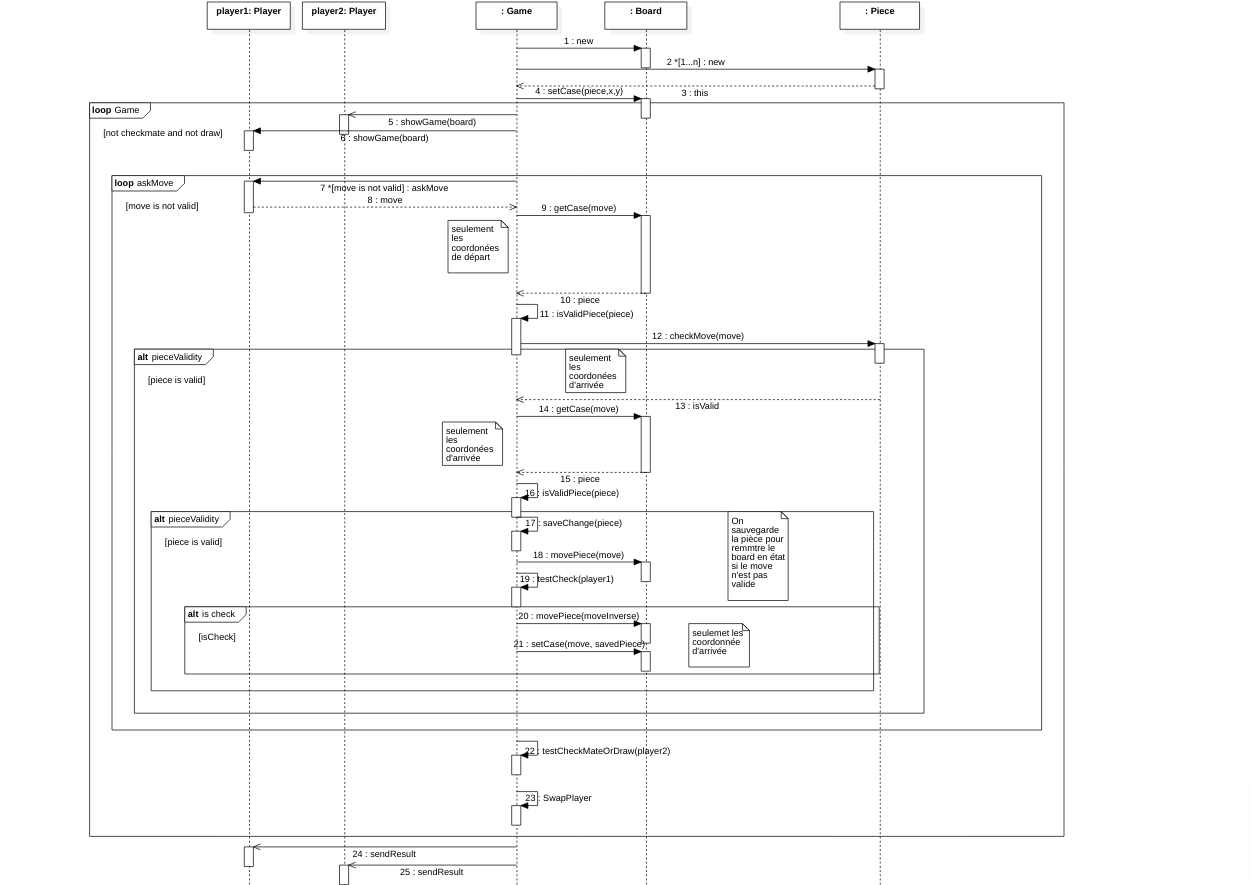
\includegraphics[scale=0.8]{SequenceDiagramClassicChessTurn.png}
\caption{Diagramme de séquence d'une partie}
\label{SD_classicgame}
\end{figure}
\clearpage



\subsubsection{Fin de la Partie}
À la fin de chaque tour, on vérifie s'il y a un gagnant ou si l'on a affaire à un Pat. Si oui, le résultat est envoyé à chacun des joueurs et la partie se termine.


\section{Besoins Systèmes : Non-Fonctionnels}


\subsection{Système d'Exploitation}
Le programme doit être capable de tourner sous Unix. \\

\subsection{Réseau}
Le jeu se joue en réseau. Une connexion internet est donc requise. \\

\subsection{Mise à Jour des Différentes Fonctionnalités}
Le système se doit de mettre assez rapidement à jour les statistiques personnelles et le classement global après chaque partie.

\section{Design du Système}

\begin{figure}[ht]
\centering
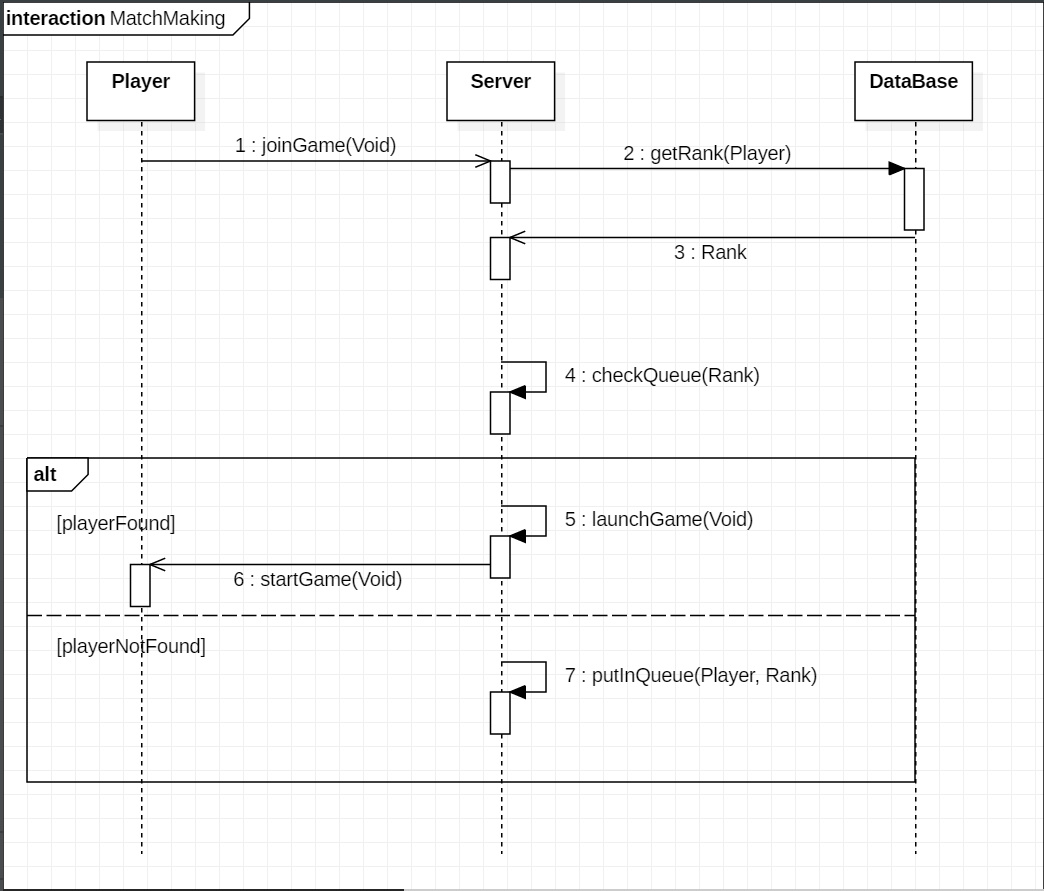
\includegraphics[scale=0.72]{SequenceDiagramMatchmaking.PNG}
\caption{Diagramme de séquence pour le \textit{Matchmaking}}
\label{SD_matchmaker} %SequenceDiagram_matchmaking
\end{figure}
\subsection{Les Différentes Classes}

\begin{sidewaysfigure}[ph]
%\centering
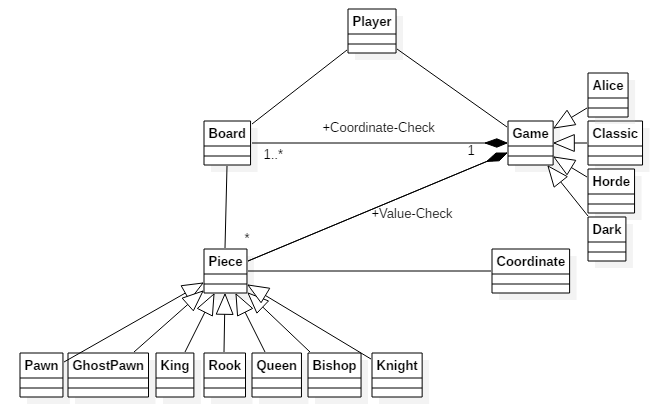
\includegraphics[scale=0.5]{ClassDiagram.png}
\caption{Diagramme de classes général}
\label{CD} %ClassDiagram
\end{sidewaysfigure}

\newpage

\subsection{Connexion du Joueur}

\subsection{Les Actions du Joueur}

\subsection{Client-Serveur}
\paragraph{}Dans le cadre de ce projet, nous avons décidé que la partie serveur s'occupera de toute la logique du jeu tandis que la partie client s'assurera d'afficher correctement l'interface du jeu en temps réel et pour se faire, enverra des requêtes au serveur pour connaître les mouvements de pièces.
\paragraph{}Il convient également de spécifier que l'échange d'information entre le serveur et le client se fera sous le format de chaînes de caractères. Par exemple, Le serveur enregistrera les noms de compte et mots de passe des joueurs dans un fichier texte et non une base de données. Et cela pour au moins 3 raisons décrites ci-dessous : 
\begin{enumerate}
\item Comme la plupart des tâches effectuées par nos programmes se font à l'aide de chaînes de caractères et par soucis d'homogénéité, il est préferable et plus simple que l'échange d'information entre le serveur et le client se fasse également sous cette forme.
\item Une chaîne de caractère n'a pas besoin d'être traduite en binaire, ce qui diminue la complexité et le temps d'exécution de nos programmes.
\item La taille du message envoyée n'est pas un probleme, car une taille de 100 octets suffit pour envoyer toutes les informations d'un message. Le plus grand message actuel est le plateau, qui ne consiste que de 98 octets lorsqu'il est complet (voir 6.5.2)
\end{enumerate}
\paragraph{}Le serveur aura une copie du board et tâchera de vérifier les différentes actions des joueurs. Il veillera également à mettre à jour les board des joueurs.

\subsection{Déroulement d'une partie  } \\ \\

\begin{enumerate}

\item \textit{Assignation de la couleur des pièces aux joueurs} \\
\textbf{Mise en pratique :} Le serveur envoie la couleur(noir ou blanc) au client. \\
\textbf{Protocole :} Le serveur envoie '1' pour la couleur 'blanc' et '0' pour 'noir'. Pour l'instant, le premier connecté reçoit la couleur 'blanc'.  

\item \textit{Affichage de l'échiquier} \\
\textbf{Mise en pratique :} Le serveur envoie le plateau aux joueurs. \\
\textbf{Protocole :} Le message est une suite de toutes les pièces présentes sur l'échiquier, chacune représentée par 3 caractères. Le premier caractère est une lettre désignant le type de la pièce considérée. Les 2 autres, sa position, en commençant par la colonne, selon la réprésentation classique d'un échiquier, c'est à dire, les rangées sont numérotées de 1 à 9 et les colonnes de "A" à "H". Les pions blancs sont séparés des noirs par '!' et à la fin des pions noirs, on ajoute un '#'. Exemple : pA2hA4rD5qC7kE1bF8!bA8qG4kD7#. L'envoi d'un plateau contenant toutes les pièces classiques est donc de 98 octets: 1 octet par caractère, 3 caractères par pièces, 32 pièces sur un plateau, soit 3*32=96, plus les 2 symboles de séparation.   

\item \textit{Numéro du tour de jeu} \\
\textbf{Mise en pratique :} Le serveur envoie le numéro du tour actuel de jeu aux joueurs.  \\
\textbf{Protocole :} A partir d'un compteur dans la boucle de jeu, le serveur envoie le chiffre au client.  

\item \textit{Tour du joueur} \\
\textbf{Mise en pratique :} Chaque client vérifie si c'est bien au tour de son joueur de jouer, si oui, celui-ci envoie en message le mouvement de la pièce au serveur. \\
\textbf{Protocole :} Le message est composé de 4 caractères, les 2 premiers sont l'emplacement du début de tour de la pièce et les 2 derniers sont la position future de la pièce demandée par le joueur.

\item \textit{Mouvement de la pièce} \\
\textbf{Mise en pratique :} Après avoir reçu la position future de la pièce indiquée par le joueur, le serveur vérifie sa validité et envoie son résultat au client. Tant que la position n'est pas validée par le serveur, le client doit renvoyer une position au serveur. Lorsque que celle-ci est validée, le serveur envoie aux 2 clients l'échiquier mis à jour.  \\
\textbf{Protocole :} Le serveur renvoie un boolée True/False. 

\item \textit{État de la partie} \\
\textbf{Mise en pratique :} Le serveur envoie un message de statut : "<fin de jeu-match nul"> ou "<continue"> \\
\textbf{Protocole :} Le serveur renvoie True pour terminer la partie ou False pour la continuer 

\item Le joueur suivant commence son tour selon la procédure ci-dessus

\item Si la partie est terminée, le joueur est déconnecté vu qu'il n'y a pas encore de menu.

NB: Ce protocole n'est pas définitif
\end{enumerate}

\subsection{Menu}

\section{Annexe}







\end{document}


o